% \documentclass{recpad2k}
\documentclass[extendedabs]{recpad2k}

%% Enter your paper number here for the review copy
\recpadreviewcopy{1}

\title{Author Guidelines for the\\ Portuguese Conference on Pattern Recognition}

% Enter the paper's authors in order
% \addauthor{Name}{email/homepage}{INSTITUTION_CODE}
\addauthor{Susan Student}{http://www.vision.inst.ac.uk/~ss}{1}
\addauthor{Petra Prof}{http://www.vision.inst.ac.uk/~pp}{1}
\addauthor{Colin Collaborator}{colin@collaborators.com}{2}

% Enter the institutions
% \addinstitution{Name\\Address}
\addinstitution{
 The Vision Institute\\
 University of Borsetshire\\
 Wimbleham, UK
}
\addinstitution{
 Collaborators, Inc.\\
 123 Park Avenue,\\
 New York, USA
}

\runninghead{Student, Prof, Collaborator}{RECPAD Author Guidelines}

% Any macro definitions you would like to include
% These are not defined in the style file, because they don't begin
% with \bmva, so they might conflict with the user's own macros.
% The \bmvaOneDot macro adds a full stop unless there is one in the
% text already.
\def\eg{\emph{e.g}\bmvaOneDot}
\def\Eg{\emph{E.g}\bmvaOneDot}
\def\etal{\emph{et al}\bmvaOneDot}

%------------------------------------------------------------------------- 
% Document starts here
\begin{document}

\maketitle

\begin{abstract}
This document demonstrates the format requirements for papers submitted
to the Portuguese Conference on Pattern Recognition.  The format is designed for
easy on-screen reading, and to print well at one or two pages per sheet.
Additional features include: pop-up annotations for
citations~\cite{Authors06,Mermin89}; a margin ruler for reviewing; and a
greatly simplified way of entering multiple authors and institutions.

{\bf All authors are encouraged to read this document}, even if you have
written many papers before.  As well as a description of the format, the
document contains many instructions relating to formatting problems and
errors that are common even in the work of authors who {\em have}
written many papers before.
\end{abstract}

%------------------------------------------------------------------------- 
\section{Introduction}
\label{sec:intro}
The proceedings of RecPad (the Portuguese Conference on Pattern Recognition) will be published only in electronic form.  This document
illustrates the required paper format, and includes guidelines on
preparation of submissions.  Papers which fail to adhere to these
requirements may be rejected at any stage in the review process.

\LaTeX\ users should use this template in order to prepare their paper.
Users of other packages should emulate the style and layout of this
example.  Note that best results will be achieved using {\tt pdflatex},
which is available in most modern distributions.

\subsection{Paper length: two pages including bibliography and title}
Papers must be 2~pages in length, {\em including} the bibliography.  Length
is counted from the bottom of the title on the first page.  Therefore, the
bibliography should begin eight lines into page ten.  This is an
approximate measure, intended to encourage brevity, but authors should keep
in mind that blatant disregard of this instruction will cause reviewers to
require greater originality and impact of the submission.  {\bf Papers which are
clearly overlength will not be reviewed}.  This includes papers where the
margins and formatting are deemed to have been significantly altered from
those laid down by this style guide.  The reason such papers will not be
reviewed is that there is no provision for supervised revisions of
manuscripts.  The reviewing process cannot determine the suitability of the
paper for presentation in nine pages if it is reviewed in twelve.

The bibliography should begin immediately after the paper text.  It may
be of any length, within reason.  It should {\em not} include
annotations, figures, or any other paraphernalia intended to subvert the
paper length requirement.

\begin{figure}
% 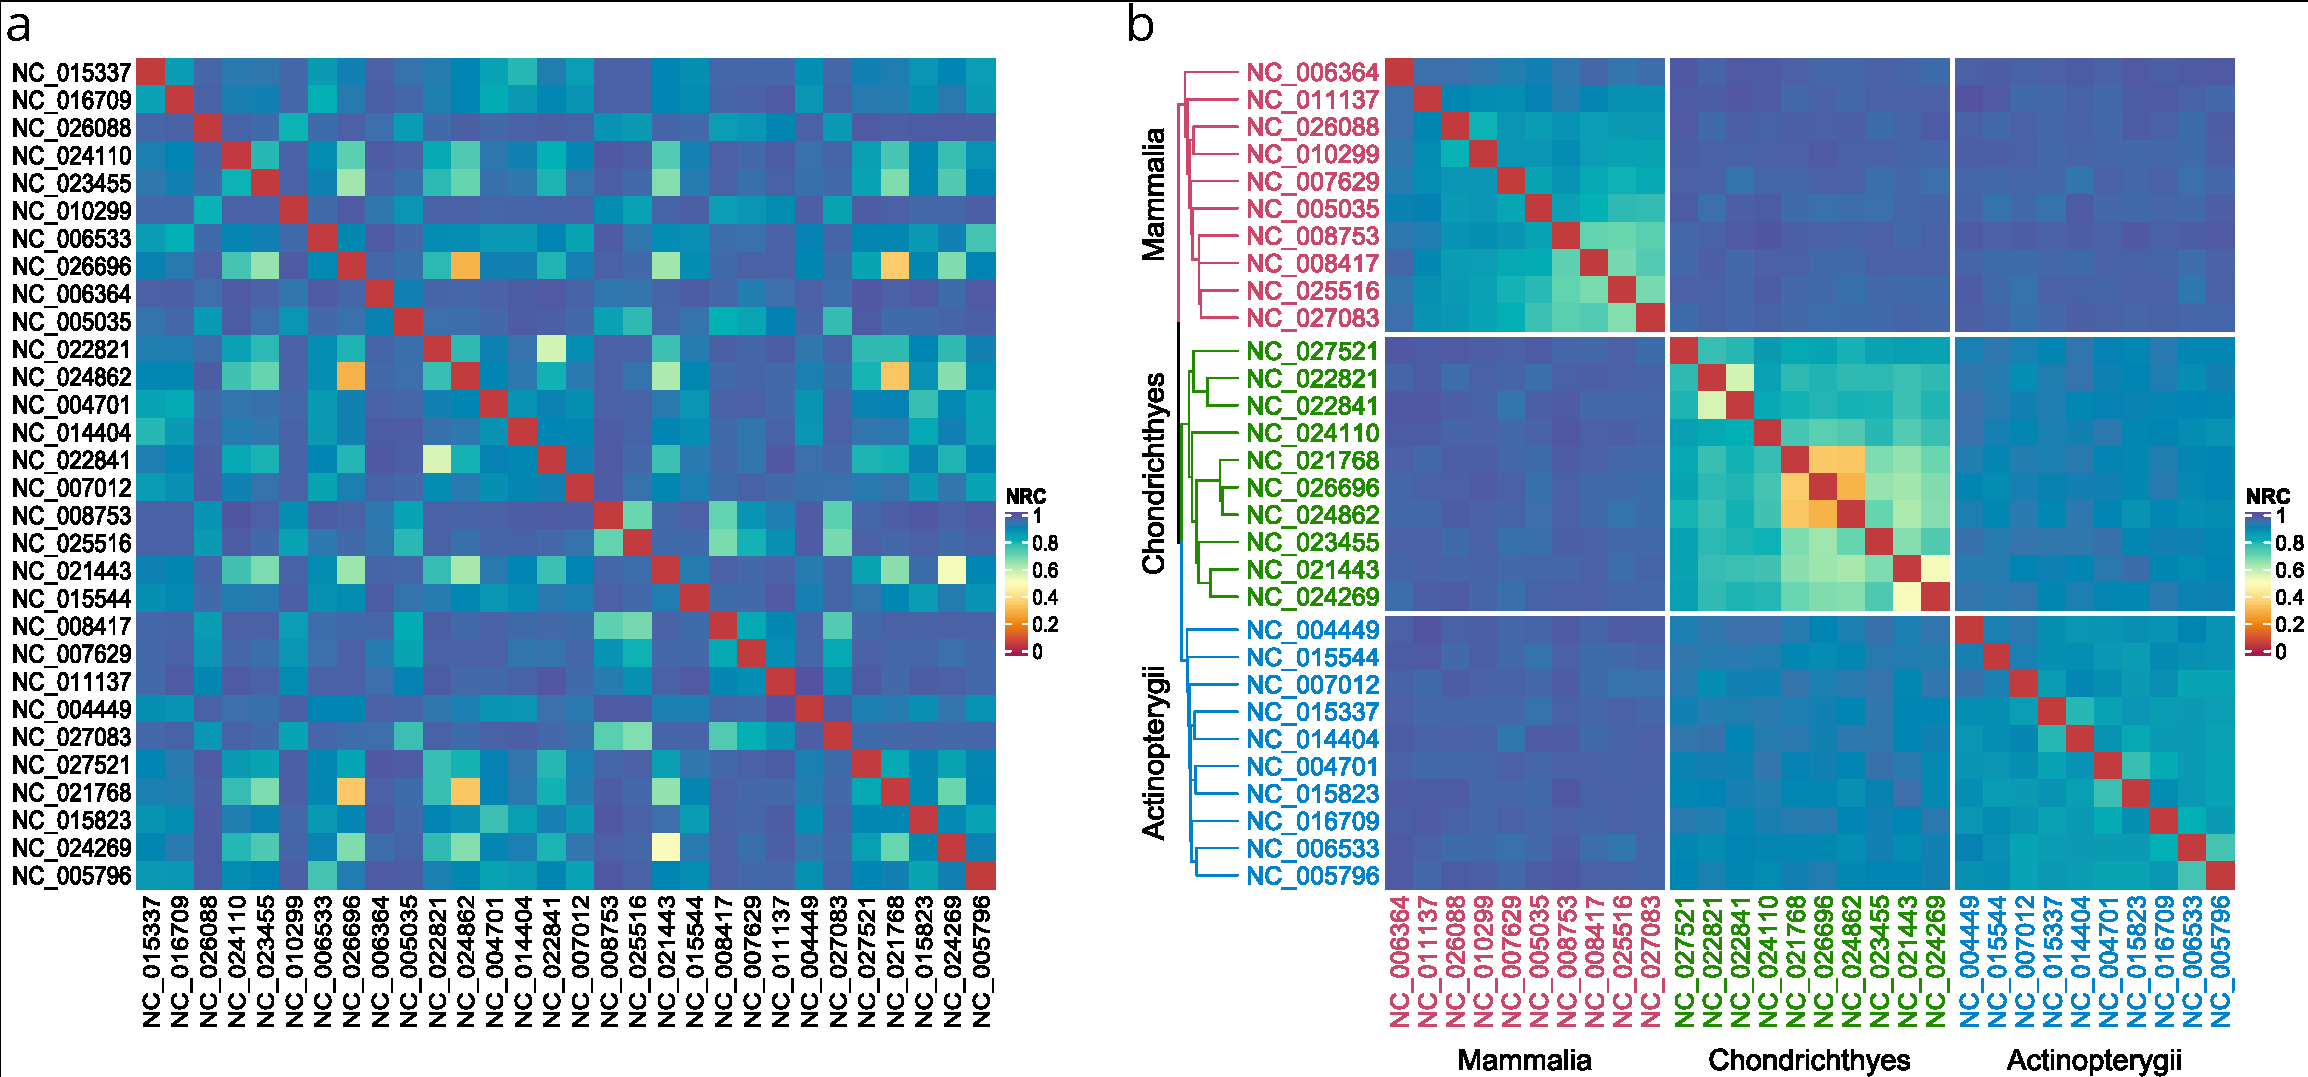
\includegraphics[width=\textwidth]{fig.pdf}
\caption{It is often a good idea for the first figure to attempt to
encapsulate the article, complementing the abstract.  This figure illustrates
the various print and on-screen layouts for which this paper format has
been optimized: (a) traditional print format; (b) on-screen
single-column format, or large-print paper; (c) full-screen two column, or
2-up printing. }
% \label{fig:teaser}
\end{figure}



% \subsection{Citations}
% When citing a multi-author paper, you may save space by using ``{\em et
% alia}'', shortened to ``\etal'' (not ``{\em et.\ al.}'' as ``{\em et}'' is
% a complete word.)  The provided \verb'\etal' macro is a useful {\em aide
% memoire} in this regard.  However, use it only when there are three or more
% authors.  Thus, the following is correct: `` Frobnication has been trendy
% lately.  It was introduced by Alpher~\cite{Alpher02}, and subsequently
% developed by Alpher and Fotheringham-Smythe~\cite{Alpher03}, and Alpher
% \etal~\cite{Alpher04}.''

% This is incorrect: ``... subsequently developed by Alpher \etal~\cite{Alpher03} ...''
% because reference~\cite{Alpher03} has just two authors.  If you use the
% \verb'\etal' macro, then you need not worry about double periods
% when used at the end of a sentence as in Alpher \etal.

% %For this citation style, keep multiple citations in numerical (not
% %chronological) order, so prefer
% We use {\tt natbib}, so citations in random order are nicely sorted:
%  \cite{Alpher03,Alpher02,Authors06b,Authors06}.  However, we don't use the
% compress option, as we want each reference to have its own hyperlink and
% popup window.

% %------------------------------------------------------------------------- 
% \subsection{Footnotes}

% Please use footnotes\footnote {This is what a footnote looks like.  It
% often distracts the reader from the main flow of the argument.} sparingly.
% Indeed, try to avoid footnotes altogether and include necessary peripheral
% observations in 
% the text (within parentheses, if you prefer, as in this sentence).  If you
% wish to use a footnote, place it at the bottom of the column on the page on
% which it is referenced. Use Times 8-point type, single-spaced.


% \begin{figure*}
% \begin{center}
% \fbox{\rule{0pt}{2in} \rule{.9\linewidth}{0pt}}
% \end{center}
%    \caption{Example of a short caption, which should be centered.}
% \label{fig:short}
% \end{figure*}

% %------------------------------------------------------------------------- 
% \subsection{The ruler}
% The \LaTeX\ style defines a printed ruler which should be present in the
% version submitted for review.  The ruler is provided in order that
% reviewers may comment on particular lines in the paper without
% circumlocution.  If you are preparing a document using a non-\LaTeX\
% document preparation system, please arrange for an equivalent ruler to
% appear on the final output pages.  The presence or absence of the ruler
% should not change the appearance of any other content on the page.  The
% camera ready copy should not contain a ruler. (\LaTeX\ users may remove
% the \verb'[review]' option from the \verb'\documentclass' statement.)
% Reviewers: note that the ruler measurements do not align well with lines
% in the paper --- this turns out to be very difficult to do well when the
% paper contains many figures and equations, and, when done, looks ugly.
% Just use fractional references (e.g.\ this line is $210.5$), although in
% most cases one would expect that the approximate location ($210$ in the
% previous example) will be adequate.


% \begin{table}
% \begin{center}
% \begin{tabular}{|l|c|}
% \hline
% Method & Frobnability \\
% \hline\hline
% Theirs & Frumpy \\
% Yours & Frobbly \\
% Ours & Makes one's heart Frob\\
% \hline
% \end{tabular}
% \end{center}
% \caption{Results.   Ours is better.}
% \end{table}

% \subsection{Mathematics}

% Please number all of your sections and displayed equations.  It is
% important for readers to be able to refer to any particular equation.  Just
% because you didn't refer to it in the text doesn't mean some future reader
% might not need to refer to it.  It is cumbersome to have to use
% circumlocutions like ``the equation second from the top of page 3 column
% 1''.  (Note that the ruler will not be present in the final copy, so is not
% an alternative to equation numbers).  All authors will benefit from reading
% Mermin's description~\cite{Mermin89} of how to write mathematics.


% %------------------------------------------------------------------------- 
% \section{References}

% List and number all bibliographical references in 9-point Times,
% single-spaced, at the end of your paper. When referenced in the text,
% enclose the citation number in square brackets, for
% example~\cite{Authors06}.  Where appropriate, include the name(s) of
% editors of referenced books.


% %------------------------------------------------------------------------
% \section{Color}

% Color is valuable, and will be visible to readers of the electronic copy.
% However ensure that, when printed on a monochrome printer, no important
% information is lost by the conversion to grayscale.

% \bibliography{egbib}
\end{document}
